\documentclass{article}

\usepackage{siunitx} % Provides the \SI{}{} command for typesetting SI units
\usepackage{graphicx} % Required for the inclusion of images
\setlength\parindent{0pt} % Removes all indentation from paragraphs
\renewcommand{\labelenumi}{\alph{enumi}.} % Make numbering in the enumerate environment by letter rather than number (e.g. section 6)

%\usepackage{times} % Uncomment to use the Times New Roman font

%----------------------------------------------------------------------------------------
%	DOCUMENT INFORMATION
%----------------------------------------------------------------------------------------

\title{SFC} % Title
\author{Batman} % Author name
\date{\today} % Date for the report
\begin{document}
\maketitle % Insert the title, author and date

\begin{center}
\begin{tabular}{l r}
Date Performed: & December 31, 2013 \\ % Date the experiment was performed
Partners: & Robin \\ % Partner names
\end{tabular}
\end{center}

% If you wish to include an abstract, uncomment the lines below
% \begin{abstract}
% Abstract text
% \end{abstract}

%----------------------------------------------------------------------------------------
%	SECTION 1
%----------------------------------------------------------------------------------------

\section{Changes}

There is no significant update in SFC side.  
We only have three changes:
\begin{enumerate}
\item A new Cisco catalyst 2960 installation in SFC's NOC. 
\item A new NAT64 server based on OpenBSD-5.4-CURRENT.
\item Routing daemon updates to Quagga-0.99.22.4 in nara-gate router. 
\end{enumerate}

Because only a new NAT64 server has big significance in our operation, we will discuss in next paragraphs.  

\begin{figure}[h!]
\centering
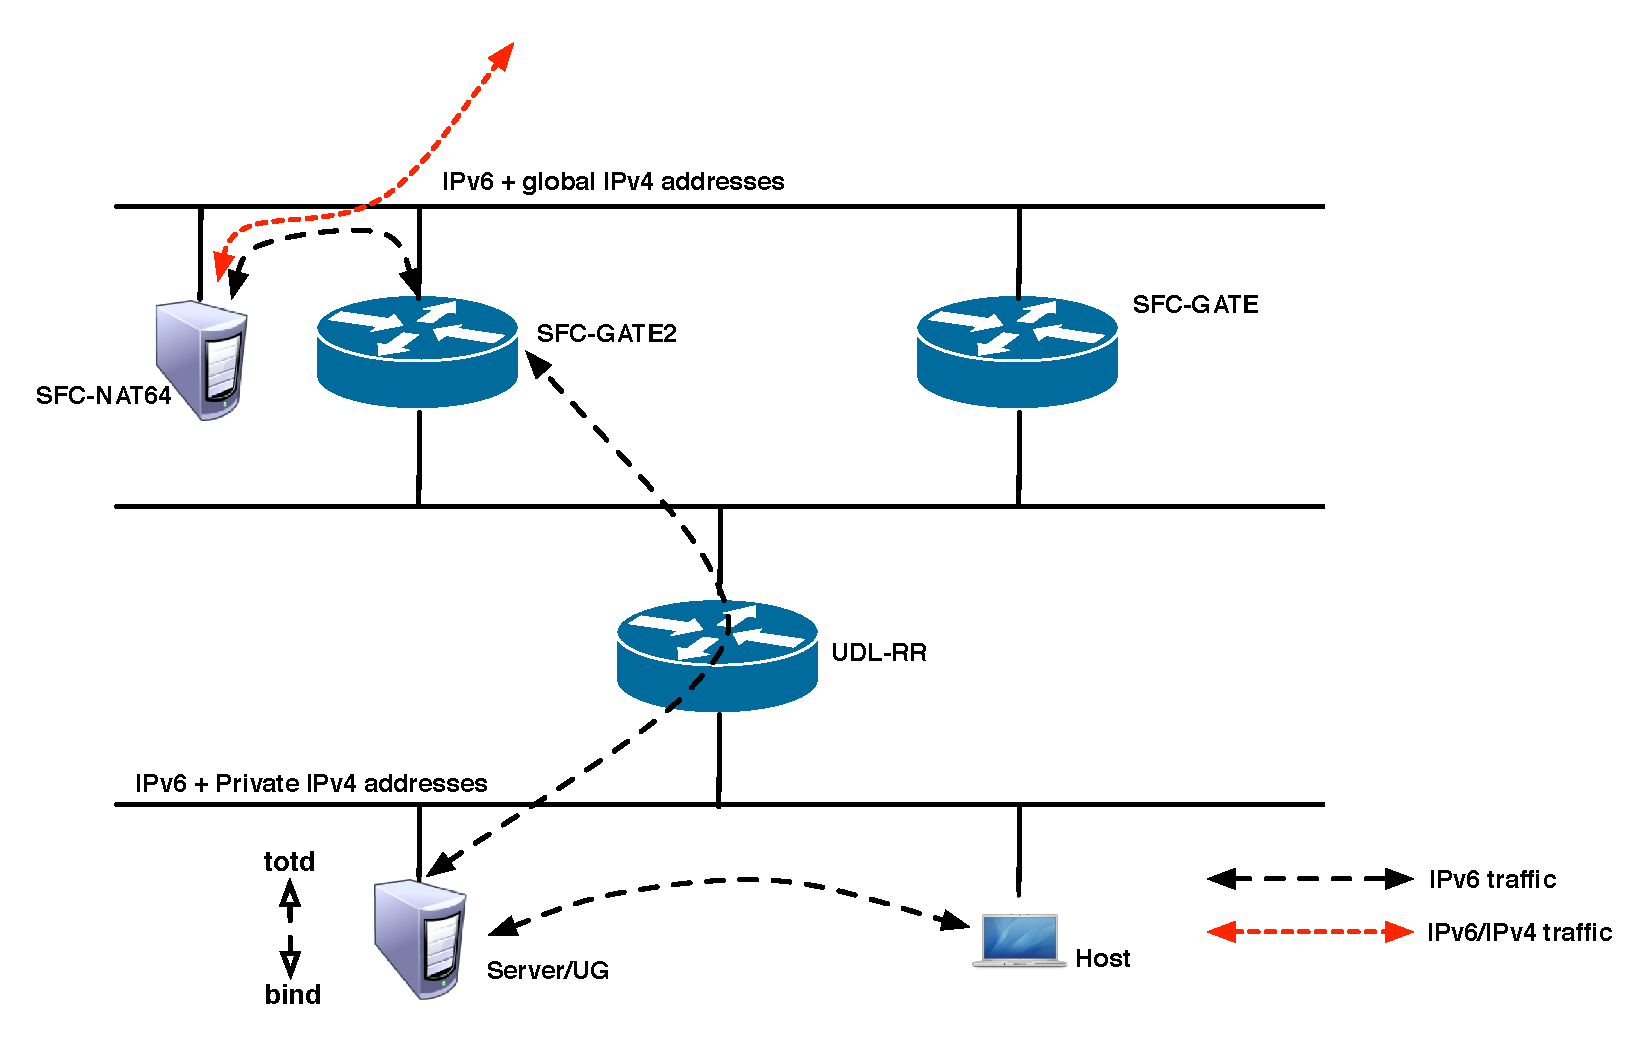
\includegraphics[width=1.\textwidth]{nat64}
\caption{Accessing IPv4 Internet via SFC-NAT64}
\label{fig:nat64}
\end{figure}

Due to un-stable of old sfc-nat64.ai3.net operation which uses naptd, we decided to change nat64 implementation from natptd to OpenBSD's nat64 implementation.  
We use OpenBSD because it is in kernel level natively support and simple configuration of translator in OpenBSD's packet filter (pf).
We also prepare backup nat64 server using Linux which uses jool kernel module from \url{https://github.com/NICMx/NAT64} in case we have trouble with OpenBSD in the future. 

Figure \ref{fig:nat64} shows how the host which has IPv6 global address and private IPv4 address can access IPv4 Internet via sfc-nat6. 
If host wants to access IPv4 website, totd daemon in server will help to translate IPv4 address of destination into IPv6 address.
AI3 uses 2001:d30:101:624::/96 IPv6 address pool for translation purpose.  
Since we added IPv6 static routing in sfc-gate2, that every 2001:d30:101:624::/96 prefix must go trough sfc-nat64, the request from server will forward to sfc-nat64 server. 





\end{document}
